\section{Singular Value Decomposition (SVD)}\label{s:svd_all}
The approach using SVD is similar to, and could even be viewed as an implementation of, the approximate nearest neighbour approach.
The application of kNN to the task of classifying images is known to suffer from various phenomena that arise when analysing high-dimensional spaces.
Problems that we have seen until now that result from this are the severely reduced effectiveness of the \(k\)-d tree and the fact that increasing \(k\) reduces accuracy.
These various phenomena are known as the curse of dimensionality~\cite{Beyer1999}.

Dimensionality reduction is the process of reducing the number of random variables under consideration~\cite{Roweis2000}.
To retain as much information as possible, the data is transformed from the high-dimensional space to a space of fewer dimensions, in a process known as feature extraction.
In this paper, the singular value decomposition~(SVD) is used. This technique is also known as the principal component analysis~(PCA) in the field of statistics.

SVD is regularly researched in the context classifying images of faces and handwritten digits~\cite{Cao2006, Savas2007}.
In this section the SVD and particularly the left-singular vectors are used to classify handwritten digits.

\subsection{Training}\label{s:svd:training}
In this subsection, several concepts of subspaces and the SVD are explained together with their role in the context of image classification.
As mentioned before, it is easier to work with images in the form of a vector as compared to a matrix or grid and therefore, images are flattened first.
Next, a matrix \(\vec{A}_n\) is created for each of the digits, such that the columns consist of all column vectors representing the number \(n\).
Suppose \(a_i\) with \(i = 1, 2, 3, \ldots, k\) are the training vectors representing the number \(n\).
The matrix has the following structure:
\[
    \vec{A}_n =
    \left(
    \begin{array}{cccc}
            \vertbar & \vertbar &        & \vertbar \\
            a_1      & a_2      & \cdots & a_k      \\
            \vertbar & \vertbar &        & \vertbar \\
        \end{array}
    \right).
\]
For example, the columns of the matrix \(\vec{A}_3\) consists of all vectors which are labelled as the number three.

The column space of a matrix \(\vec{A}\) is a space containing all linear combinations of its column vectors.
The column space of \(\vec{A}\) is also called the image or range, \(\mathcal{R}(\vec{A})\), of \(\vec{A}\).
The set of all possible linear combinations is also called the (linear) span or linear hull.

The column space of \(\vec{A}_n\) is now a space containing all linear combinations of the images that represent the number \(n\).
Each number has a subspace of the pixel space associated with it.
This can already be used for classification.
All that needs to be done is to calculate this distance between the test image and all linear subspaces. The number associated with the subspace that is closest to the test image is chosen as the label of the test image.

Each linear subspace is spanned by a lot of vectors.
This results in a very expensive distance computation and a lot of overlap of the different subspaces.
An image that is in both subspaces will have a distance of zero to both, so overlapping subspaces are guaranteed to result in worse accuracy.

This way of classifying is thus both very slow and inaccurate.
To improve this, the SVD will be used to find vectors that span smaller subspaces.

\textbf{Theorem. (SVD)} \textit{Any matrix \(\vec{A}\in \mathbb{R}^{m \times n}\), with \(m\geq n\) can be factorised
    \[\vec{A} = \vec{U}\vec{\Sigma}\vec{V}^T,\]
    where \(\vec{U}\in\mathbb{R}^{m\times m}\) and \(\vec{V}\in\mathbb{R}^{n\times n}\) orthogonal, and \(\vec{\Sigma}\in\mathbb{R}^{m\times n}\) is rectangular diagonal,
    \[\Sigma = \textnormal{diag}(\sigma_1, \sigma_2, \ldots, \sigma_n),\]
    \[\sigma_1\geq\sigma_2\geq\cdots\geq\sigma_n\geq 0.\]
    The values on the diagonal of the matrix \(\vec{\Sigma}\) are known as the singular values, while the columns of \(\vec{U}\) and \(\vec{V}\) are called the left-singular and right-singular vectors respectively~\cite{Elden2011, Savas2007}.}

The derivation below shows that the left-singular vectors are the set of eigenvectors of \(\vec{A}\vec{A}^T\).
These are thus obtained by solving the eigenvalue problem \(\vec{A}\vec{A}^T\vec{x} = \sigma \vec{x}\).
\begin{align*}
    \vec{A}                      & = \vec{U}\vec{\Sigma}\vec{V}^T                                 \\
    \vec{A}^T                    & = \vec{V}\vec{\Sigma}^T\vec{U}^T                               \\
    \Rightarrow \vec{A}\vec{A}^T & = \vec{U}\vec{\Sigma}\vec{V}^T\vec{V}\vec{\Sigma}^T\vec{U}^T   \\
    \Rightarrow \vec{A}\vec{A}^T & = \vec{U}\vec{\Sigma}(\vec{V}^T\vec{V})\vec{\Sigma}^T\vec{U}^T \\
    \Rightarrow \vec{A}\vec{A}^T & = \vec{U}(\vec{\Sigma}\vec{\Sigma}^T)\vec{U}^T
\end{align*}
\(\vec{\Sigma}\vec{\Sigma}^T\) is a real symmetric matrix, so the eigenvectors can be chosen to be orthogonal.
The remainder of this section assumes that the eigenvectors are orthonormal, which is obtained by dividing the eigenvectors by their norm.

We define \(p\) as the rank of \(\vec{A}\), then we have the following:
\begin{align*}
    \mathcal{R}(\vec{A}) & = \{\vec{A}\vec{x}:\vec{x}\in\mathbb{R}^n\}                      \\
                         & = \{\vec{U}\vec{\Sigma}\vec{V}^T\vec{x}:\vec{x}\in\mathbb{R}^n\} \\
                         & = \{\vec{U}\vec{\Sigma}\vec{y}:\vec{y}\in\mathbb{R}^n\}          \\
                         & = \{\sum_{j = 1}^n \vec{u}_j c_j:c_j\in\mathbb{R}\}            \\
                         & = \mathcal{R}(\left(\begin{array}{cccc}
            \vertbar & \vertbar &        & \vertbar \\
            u_1      & u_2      & \cdots & u_p      \\
            \vertbar & \vertbar &        & \vertbar \\
        \end{array}\right)).
\end{align*}
This means that the first \(n\) columns of \(\vec{U}\) form an orthonormal basis for \(\mathcal{R}(\vec{A})\), that is the first \(k\) columns of \(\vec{U}\) are orthogonal and they are all unit vectors~\cite{Cao2006}.
In Section~\ref{s:svd} the importance of orthonormality will be explained.
To clarify, the first \(k\) columns of \(\vec{U}_n\) form the orthonormal basis, so from this point onwards \(\vec{U}_n\) refers to the first \(p\) columns of \(\vec{U}_n\).

The fact that the singular values are in decreasing order means that the corresponding left-singular vectors are in decreasing order of importance.
Intuitively, the first \(k\) columns of \(\vec{U}\) span a space using the \(k\) most important orthogonal directions.
The first three columns of \(\vec{U}_3\) are visible in Figures~\ref{fig:svd_u1},~\ref{fig:svd_u2}~and~\ref{fig:svd_u3}.

\begin{figure}[H]
    \centering
    \begin{minipage}{0.3\textwidth}
        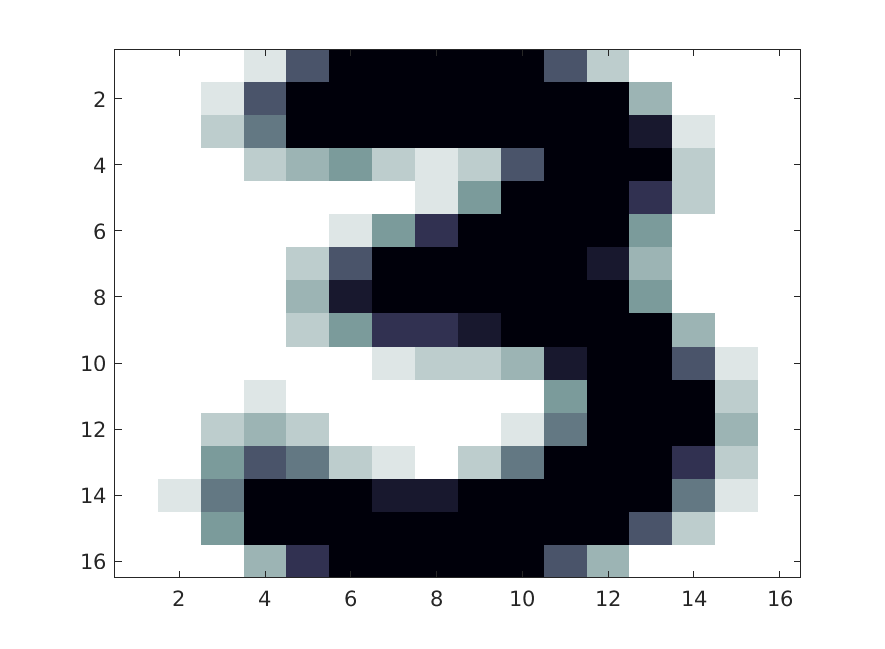
\includegraphics[width = \textwidth]{images/svd/U1.png}
        \caption{Column 1 of \(\vec{U}_3\).}\label{fig:svd_u1}
    \end{minipage}
    \begin{minipage}{0.3\textwidth}
        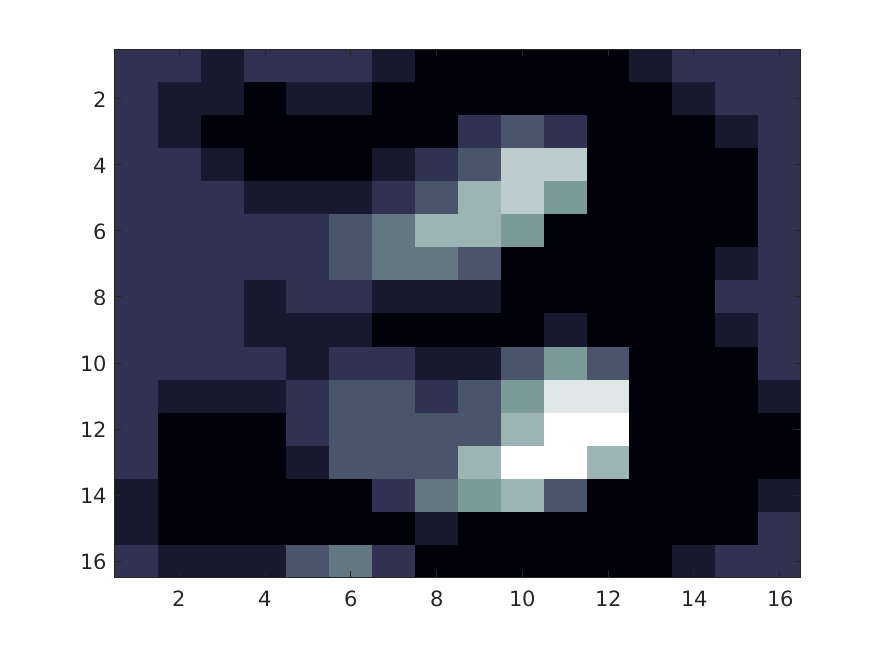
\includegraphics[width = \textwidth]{images/svd/U2.png}
        \caption{Column 2 of \(\vec{U}_3\).}\label{fig:svd_u2}
    \end{minipage}
    \begin{minipage}{0.3\textwidth}
        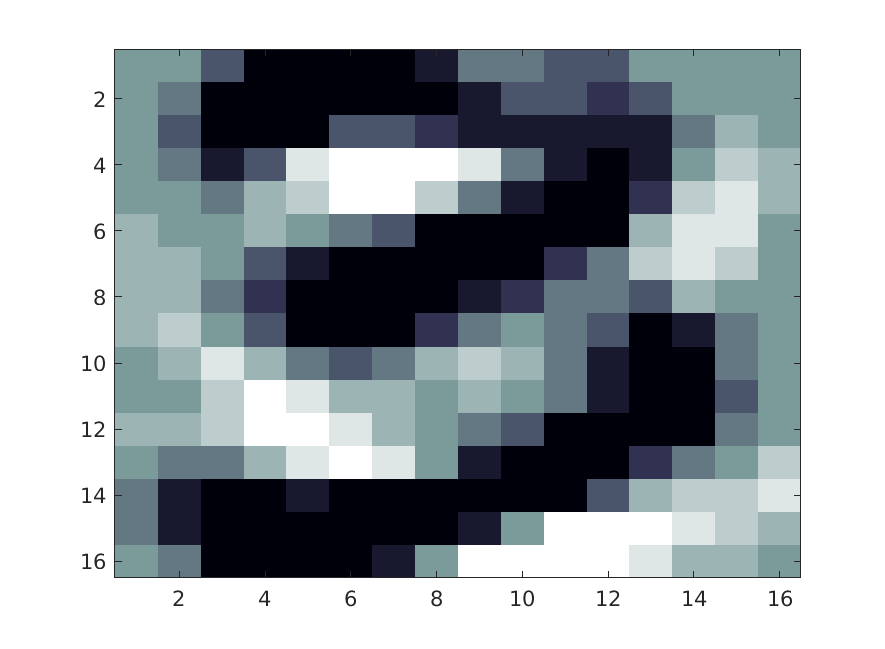
\includegraphics[width = \textwidth]{images/svd/U3.png}
        \caption{Column 3 of \(\vec{U}_3\).}\label{fig:svd_u3}
    \end{minipage}
\end{figure}

In this section several concepts were explained and how they are useful in the context of image classification.
In the next subsection these concepts, and the SVD in particular, together with some mathematical operations will be used to identify the images from the test set.

\subsection{Classification}
In this section the classification procedure using these ideas is explained in more detail and more information is given with regard to finding the distance to a linear subspace.

\subsubsection{Subspace spanned by training vectors}
The distance between an image and a subspace cannot be computed directly.
To do this, the distance between an image and its orthogonal projection on the subspace needs to be calculated instead.

\begin{figure}[H]
    \centering
    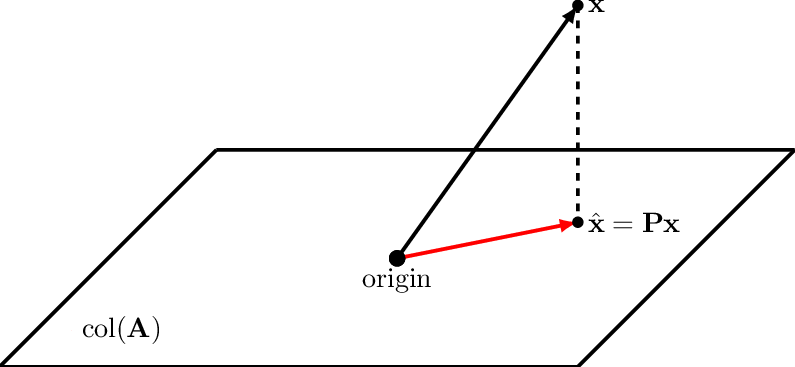
\includegraphics[width = 0.6\textwidth]{images/svd/orth_proj.png}
    \caption{Orthogonal projection on the column space of \(\vec{A}\), or col\((\vec{A})\)~\cite{Erichson2016}.}\label{fig:orth_proj}
\end{figure}

Suppose that \(\vec{x}\) is the vector that needs to be classified and that \(\hat{\vec{x}} = \vec{P}_n\vec{x}\) is the orthogonal projection of \(\vec{x}\) on the subspace representing the number \(n\).
The distance between \(\vec{x}\) and \(\hat{\vec{x}}\) is (see Figure~\ref{fig:orth_proj})
\[\norm{\vec{x} - P\vec{x}} = \big\lVert\vec{x} - \vec{A}_n{(\vec{A}_n^T \vec{A}_n)}^{-1}\vec{A}_n^T\vec{x}\big\rVert_2. \]

For each new vector the distance to each subspace is calculated.
Suppose that the closest subspace is \(\mathcal{R}(\vec{A}_n)\), which would mean that \(\vec{x}\) is classified as the number \(n\).
Notice that the column space of \(\vec{A}_n\) must be spanned by linearly independent vectors for the inverse of \(\vec{A}_n^T \vec{A}_n\) to exist.

Intuitively, the linear projection of a vector is in fact the best approximation of the vector using a linear combination of the basis vectors.
An image representing the number three (Figure~\ref{fig:svd_test3}) and number nine (Figure~\ref{fig:svd_test9}) can be found below.
To see how this projection affects the image, the orthogonal projections on the column space of \(\vec{A}_3\) of those numbers can be found besides them in Figures~\ref{fig:svd_test3_proj}~and~\ref{fig:svd_test9_proj} respectively.
Note that both Figure~\ref{fig:svd_test3}~and~\ref{fig:svd_test9} are not from the training set, since a projection of a training image representing the number \(n\) on the range of \(\vec{A}_n\) is just the vector itself.

\begin{figure}[H]
    \centering
    \begin{minipage}{0.45\textwidth}
        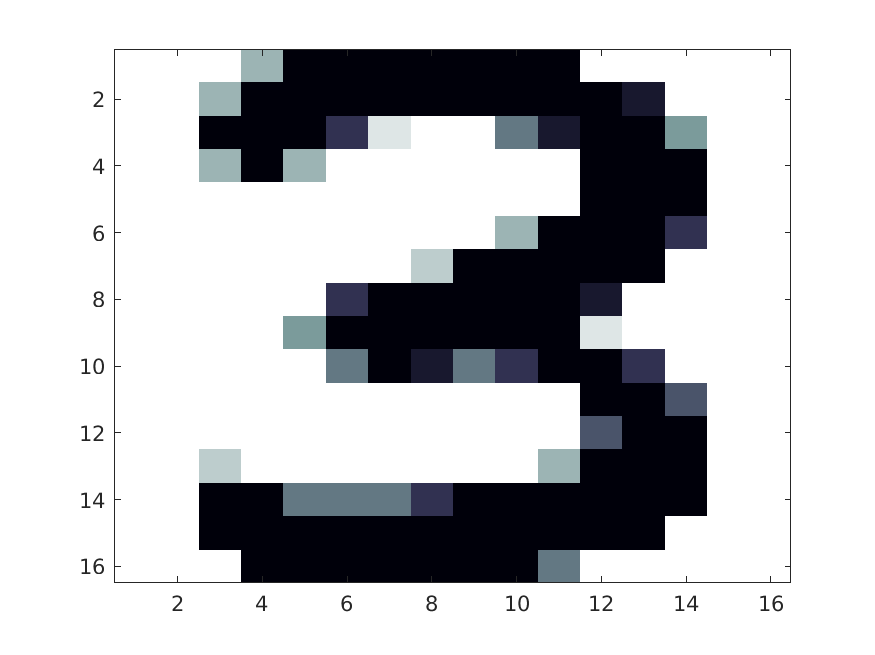
\includegraphics[width = \textwidth]{images/svd/test3.png}
        \caption{Image representing a 3 from the test set.}\label{fig:svd_test3}
    \end{minipage}
    \hspace{1em}
    \begin{minipage}{0.45\textwidth}
        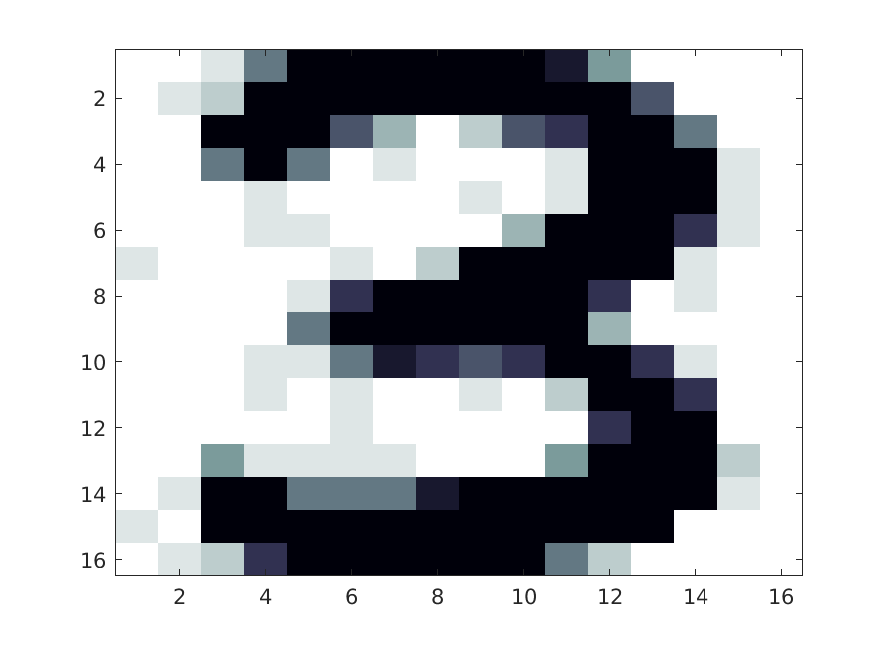
\includegraphics[width = \textwidth]{images/svd/test3_proj.png}
        \caption{Orthogonal projection of Figure~\ref{fig:svd_test3} on the range of \(\vec{A}_3\).}\label{fig:svd_test3_proj}
    \end{minipage}
\end{figure}
\begin{figure}[H]
    \begin{minipage}{0.45\textwidth}
        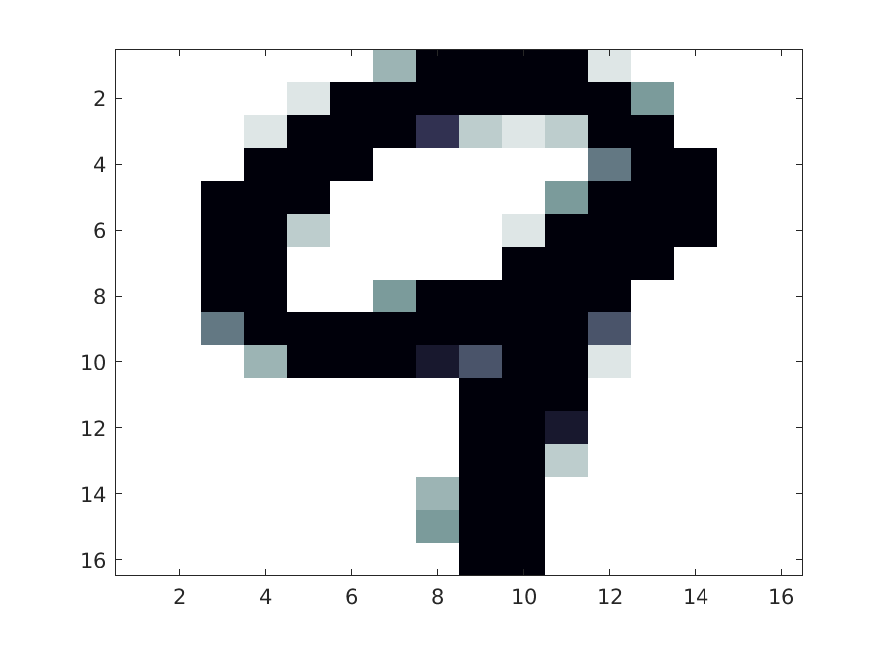
\includegraphics[width = \textwidth]{images/svd/test9.png}
        \caption{Image representing a 9 from the test set.}\label{fig:svd_test9}
    \end{minipage}
    \hspace{1em}
    \begin{minipage}{0.45\textwidth}
        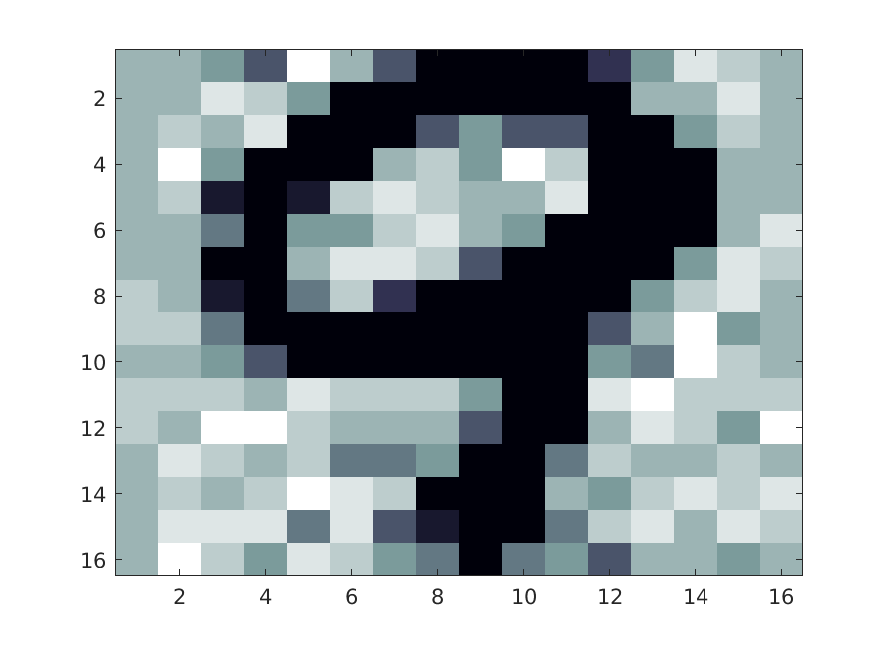
\includegraphics[width = \textwidth]{images/svd/test9_proj.png}
        \caption{Orthogonal projection of Figure~\ref{fig:svd_test9} on the range of \(\vec{A}_3\).}\label{fig:svd_test9_proj}
    \end{minipage}
\end{figure}

Recall that the column space of \(\vec{A}_3\) contains all linear combinations of the training images representing a three.
We expect there to be a linear combination closely matching the number three, while no such combination for the number nine exists.
Figures~\ref{fig:svd_test3_proj}~and~\ref{fig:svd_test9_proj} confirm this expectation as the projection of an image representing the number three on \(\mathcal{R}(\vec{A}_3)\) yields a very similar image to the original, while projecting a nine on this space introduces a lot of noise.

\subsubsection{Using the SVD}\label{s:svd}
The first step to classify digits using the SVD is to create the same matrices \(\vec{A}_n\) for each digit \(n\) as created before.
We define \(k_n\) as rank\((\vec{A}_n)\), avoiding having to write rank\((\vec{A}_n)\) everywhere.
As mentioned in Section~\ref{s:svd:training}, the singular value decomposition of each \(\vec{A}_n\) results in the matrix \(\vec{U}_n\), which is a \(256\times k_n\) matrix whose columns span \(\mathcal{R}(\vec{A}_n)\).
Hence, the columns of \(\vec{U}_n\) are \(u_1, \ldots, u_{k_n}\).
So \(\vec{U}_n^T\) and \(\vec{U}_n\) are:
\begin{align*}
    \vec{U}_n^T = \left(
    \begin{array}{ccc}
            \horzbar & u_1^T    & \horzbar \\
            \horzbar & u_2^T    & \horzbar \\
                     & \vdots &          \\
            \horzbar & u_{k_n}^T  & \horzbar
        \end{array}
    \right),
     &  &
    \vec{U}_n = \left(\begin{array}{cccc}
            \vertbar & \vertbar &        & \vertbar \\
            u_1      & u_2      & \cdots & u_{k_n}    \\
            \vertbar & \vertbar &        & \vertbar
        \end{array}
    \right).
\end{align*}
As mentioned before, the column vectors of \(\vec{U}_n\) are all orthogonal and unit vectors.
This means that \(u_i \cdot u_i = 1\) and \(u_i \cdot u_j = 0\) for all \(i \neq j\), where \(\cdot \) denotes the dot product.
The matrix multiplication of \(\vec{U}_n^T\) and \(\vec{U}_n\) then yields:
\begin{align*}
    \vec{U}_n^T \vec{U}_n & = \left(
    \begin{array}{cccc}
            u_1\cdot u_1   & u_1\cdot u_2   & \cdots & u_1\cdot u_{k_n}   \\
            u_2\cdot u_1   & u_2\cdot u_2   & \cdots & u_2\cdot u_{k_n}   \\
            \vdots         &                & \ddots & \vdots           \\
            u_{k_n}\cdot u_1 & u_{k_n}\cdot u_2 & \cdots & u_{k_n}\cdot u_{k_n}
        \end{array}\right) \\
                          &
    = \left(\begin{array}{cccc}
            1      & 0 & \cdots & 0      \\
            0      & 1 & \cdots & 0      \\
            \vdots &   & \ddots & \vdots \\
            0      & 0 & \cdots & 1
        \end{array}
    \right)                           \\
                          & = I
\end{align*}

Substituting this in the formula for the distance between a vector and its orthogonal projection yields:
\begin{align*}
    \norm{\vec{x} - P\vec{x}} & = \big\rVert\vec{x} - \vec{U}_n{(\vec{U}_n^T \vec{U}_n)}^{-1}\vec{U}_n^T\vec{x}\big\rVert \\
                              & = \norm{\vec{x} - \vec{U}_n I^{-1}\vec{U}_n^T\vec{x}}                                     \\
                              & = \norm{\vec{x} - \vec{U}_n\vec{U}_n^T\vec{x}}
\end{align*}
Therefore, the distance between a vector and a subspace spanned by the columns of \(\vec{U}_n\) is\\ \(\norm{\vec{x} - \vec{U}_n\vec{U}_n^T\vec{x}}\).

In Table~\ref{tab:nr_of_basis}, the subspace corresponding to each number is stated with the amount of basis vectors and the amount of column vectors of \(\vec{A}_n\).
Note that the training set for some numbers has an equal amount of basis vectors compared to orthonormal vectors.
This means that every vector in \(\vec{A}_n\) was already linearly independent.
\begin{table}[H]
    \centering
    \caption{Number of basis vectors used to span the different subspaces.}\label{tab:nr_of_basis}
    \begin{tabular}{lcccccccccc}
        \toprule
        \textbf{\textit{n}}                                         & 0   & 1   & 2   & 3   & 4   & 5   & 6   & 7   & 8   & 9   \\
        \textbf{\(k_n\)} & 245 & 100 & 202 & 131 & 122 & 88 & 151 & 166 & 144 & 132 \\
        \textbf{number of columns \(\vec{A}_n\)}       & 319 & 252 & 202 & 131 & 122 & 88  & 151 & 166 & 144 & 132 \\
        \bottomrule
    \end{tabular}
\end{table}
\subsection{Performance}
The difference in speed between using linearly independent columns of \(\vec{A}_n\) and the orthonormal columns of \(\vec{U}_n\) consists of two main parts.
First, the basis columns of \(\vec{A}_n\) must be chosen. To do this, each column vector needs to be checked whether or not they are a linear combination of the previous columns.
This is an expensive computation when compared to computing the SVD.\@
The second part responsible for the difference is the distance function. In Section~\ref{s:svd} we saw that the orthonormality condition resulted in a simplified calculation.
In Table~\ref{tab:svd_all} the difference between the running time of both distances can be seen.

At this point, all the columns of \(\vec{U}_n\) are used to span the space on which the vectors are projected.
As mentioned before, the singular vectors are ordered from important to less important.
The first \(r\) vectors of \(\vec{U}_n\) span a subspace of \(\mathcal{R}(\vec{A})\) that contains the most important features for the number \(n\).
A feature then is a certain combination of pixel values.
The amount of orthogonal vectors \(r\) to be taken as our basis is yet to be determined.

The choice for \(r\) must be independent from the test set, so different amounts of vectors are tested on the training set and their results are plotted in Figure~\ref{fig:r_values_acc}.
A projection onto a subspace spanned by more elements naturally has a higher computational cost.
Figure~\ref{fig:r_values_time} shows a clear upwards trend with respect to the time the algorithm takes.
The slight peak in Figure~\ref{fig:r_values_time} can be explained by caching optimisations between subsequent runs and would disappear when repeating this test multiple times.

\begin{figure}[H]
    \centering
    \begin{minipage}{0.45\textwidth}
        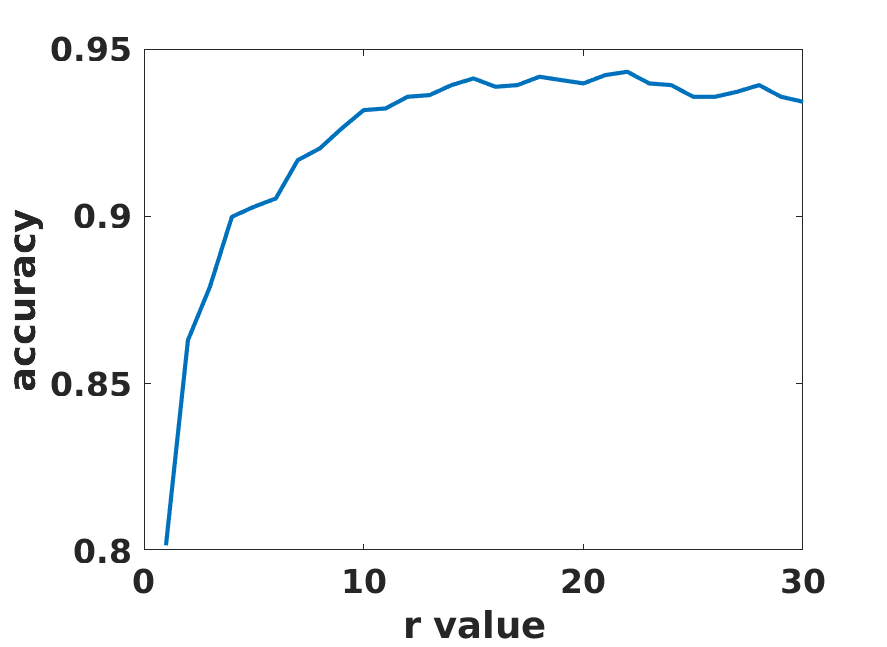
\includegraphics[width = \textwidth]{images/svd/r_values.png}
        \caption{Accuracy plotted against \(r\) values.}\label{fig:r_values_acc}
    \end{minipage}
    \begin{minipage}{0.45\textwidth}
        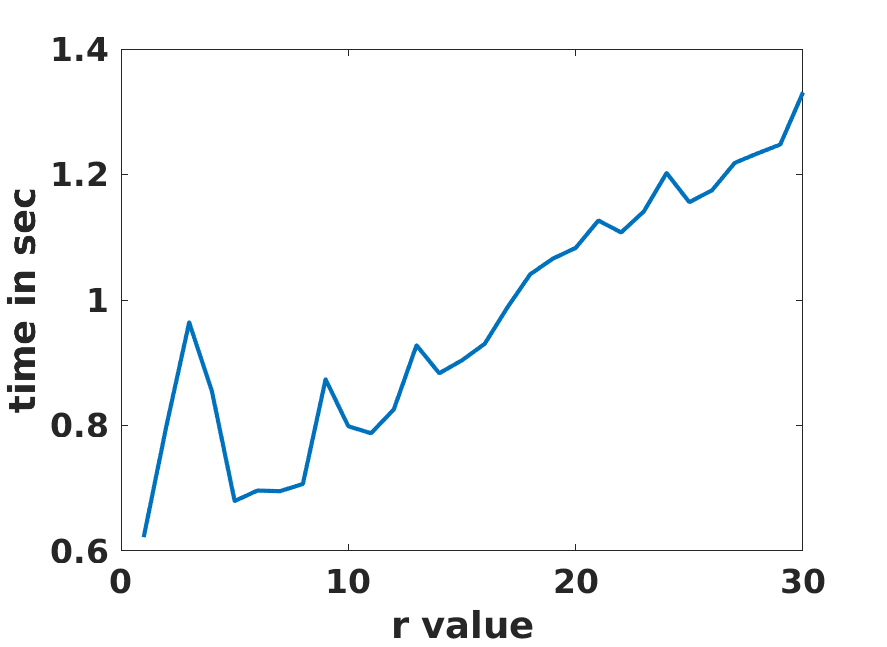
\includegraphics[width = \textwidth]{images/svd/time.png}
        \caption{Time plotted against \(r\) values.}\label{fig:r_values_time}
    \end{minipage}
\end{figure}

For a better overview, some data values at different intervals can be found in Table~\ref{tab:svd_all}.
The time difference between the simplified distance based on the orthonormality condition and the standard linear independence can also be seen here.
The graph in Figure~\ref{fig:r_values_acc} indicates that \(r = 15\) strikes a good balance between speed and accuracy.

\begin{table}[H]
    \centering
    \caption{Results of SVD classifier.}\label{tab:svd_all}
    \begin{tabular}{lccccccc}
        \toprule
        \textbf{\(r\) value} & 1    & 2    & 5    & 10   & 15   & 20   & 25   \\
        \textbf{Accuracy}    & 0.80 & 0.86 & 0.90 & 0.93 & 0.94 & 0.94 & 0.94 \\
        \textbf{Time orthonormal (s)}    & 0.62 & 0.80 & 0.68 & 0.80 & 0.90 & 1.08 & 1.16 \\
        \textbf{Time linear independent (s)}    & 1.17 & 1.57 & 1.86 & 2.19 & 2.58 & 3.23 & 3.95 \\
        \bottomrule
    \end{tabular}
\end{table}

The last two sections, kNN and SVD, tried to classify digits by computing the distance between a new image and other objects to determine the label.
Another entirely different way of doing this is by constructing a model based on the training images.
In the next section a neural network will be used to label the image.